\documentclass{beamer}

\usepackage{lmodern}

\usepackage{listings}

\usepackage[T2A]{fontenc}
\usepackage[utf8]{inputenc}

\usetheme{Madrid}
\usecolortheme{beaver}

\title[Erlang]{Исследование эффективности реализации\\некоторых структур данных на языке Erlang}
\subtitle[ПМИ]{Прикладная математика и информатика}

\author[Быцюк В.В.]{Быцюк Владислав Вячеславович}
\date[Брагилевский В.Н.]{Научный руководитель:\\старший преподаватель Брагилевский В.Н.}

\begin{document}
	\setbeamertemplate{caption}{\raggedright\insertcaption\par}

	% Титульный лист
	\begin{frame}
		\titlepage
	\end{frame}

	% Постановка задачи
	\begin{frame}{\LARGE \textbf{Постановка задачи}}
		\begin{itemize}
			\item Реализовать структуру данных <<упорядоченное множество>> на языке программирования Erlang.
			\item Сравнить время выполнения основных операций реализованной структуры данных с реализациями из модулей
			  	  ordsets и sets. 
		\end{itemize}
	\end{frame}
	
	
	% Основное содержание

	\begin{frame}[fragile]{Красно-черное дерево и Erlang}
		\begin{figure}
			\includegraphics[scale=1]{img/tree.png}
		\end{figure}
		
		\begin{block}{Реализация на Erlang}
																																																												\begin{lstlisting}  
	{Y, 
	 red, 
	 {X, black, a, b}, 
	 {Z, black, c, d}
	};		   
			\end{lstlisting}
		\end{block}	
	\end{frame}
	
	\begin{frame}[fragile]{Пример реализации проверки на то, является ли одно упорядоченное множество подмножеством другого}
		\begin{block}{Реализация на Erlang}
			\begin{lstlisting}[language = erlang] 	
is_subset({nil, black, nil, nil}, _) ->
    true;	
	
is_subset({Key, _, Left, Right}, OSetB) ->
    IsElem = is_element(Key, OSetB),
    if
        IsElem  -> is_subset(Left, OSetB) 
                   and 
                   is_subset(Right, OSetB);
        true    -> false
    end.
			\end{lstlisting}
		\end{block}	
	\end{frame}
	
	\begin{frame}{Сравнение времени выполнения}
		Сравнение происходит следующим образом:
		\begin{itemize}
			\item Генерируется текстовый файл со 100 000 целых чисел
			\item Считываются данные из файла в структуру данных
			\item Проводятся несколько замеров времени выполнения для каждой операции
			\item Выводится среднее время выполнения для каждой операции
		\end{itemize}
	\end{frame}
	
	\begin{frame}{Сравнение времени выполнения на примере операции вставки}
		\begin{figure}
			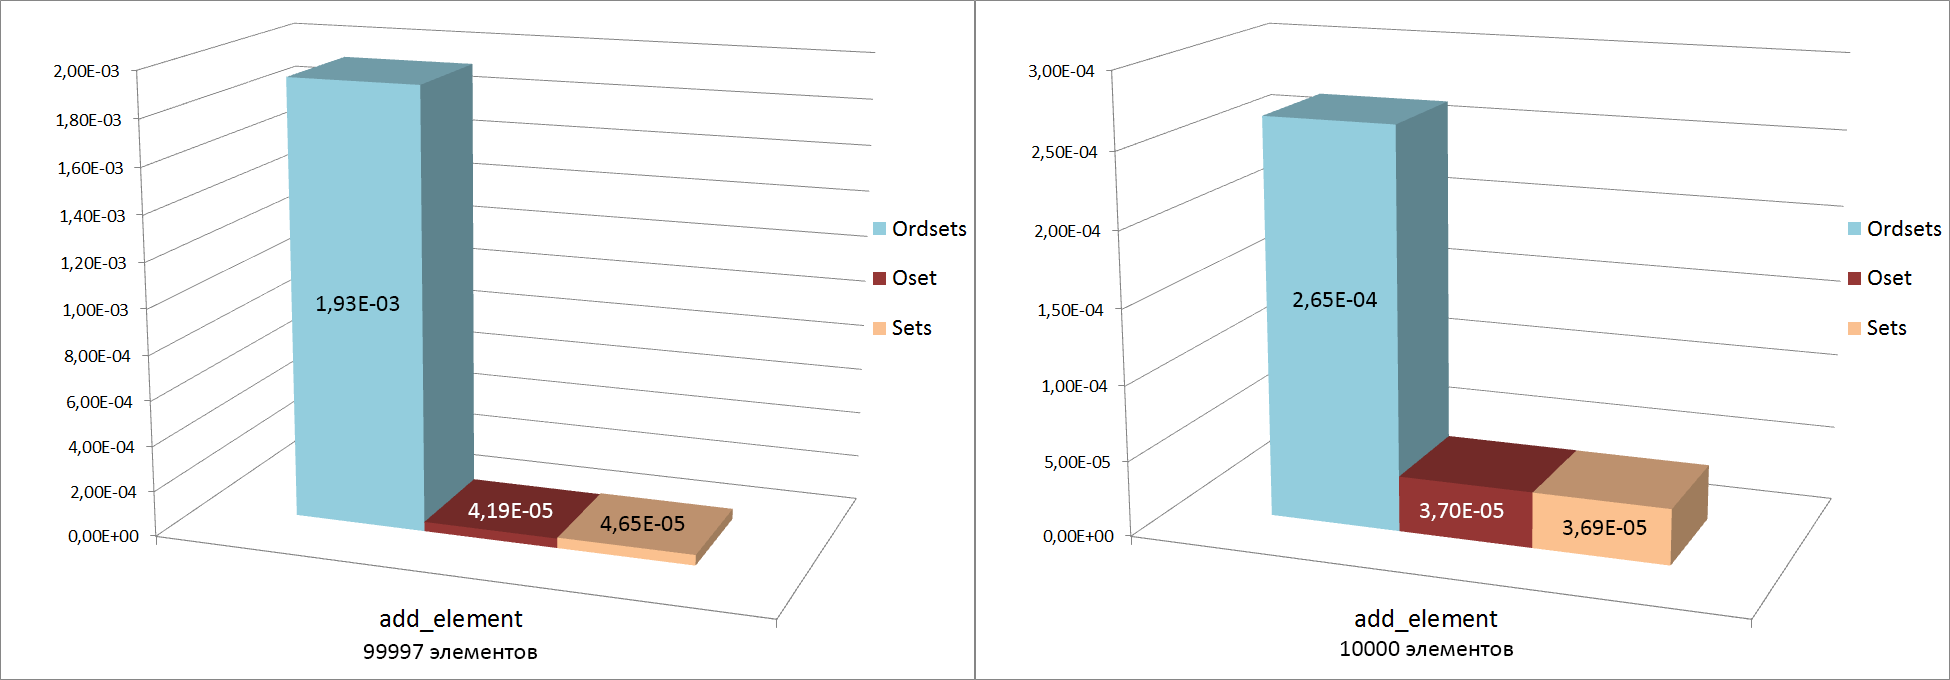
\includegraphics[scale=0.18]{img/histograms/add_element.png}
			\caption{Вставка}
		\end{figure}
	\end{frame}
	
	
	\begin{frame}{Сравнение времени выполнения на примере одной логической операции}				
		\begin{figure}
			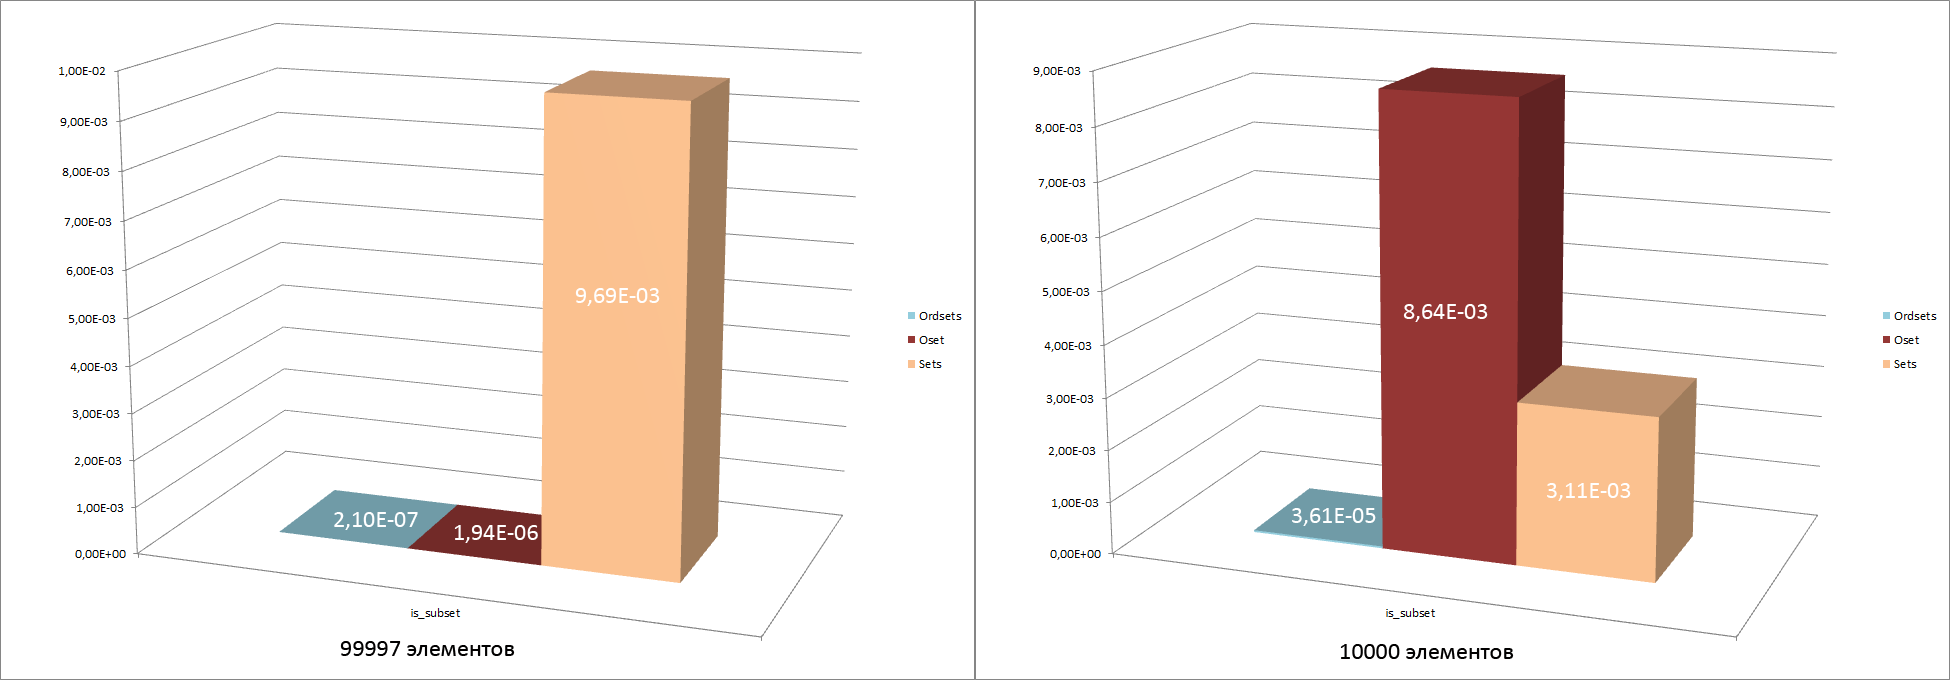
\includegraphics[scale=0.18]{img/histograms/is_subset.png}
			\caption{Проверка на то, является ли одно упорядоченное множество подмножеством другого}
		\end{figure}
	\end{frame}
	
	\begin{frame}{Сравнение времени выполнения на примере операции пересечения}
		\begin{figure}
			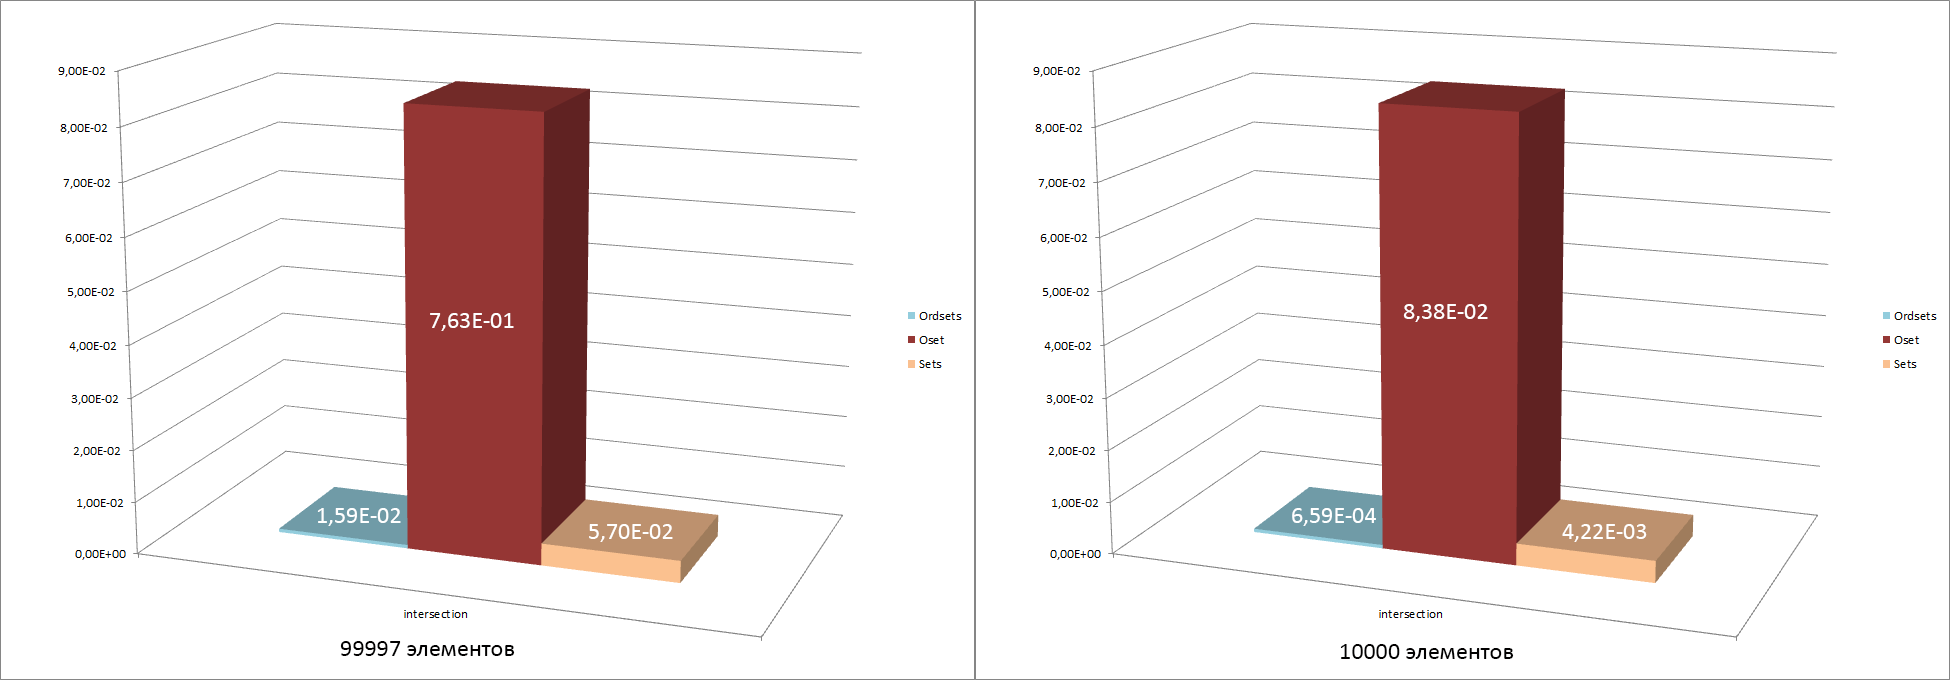
\includegraphics[scale=0.18]{img/histograms/intersection.png}
			\caption{Пересечение}
		\end{figure}		
	\end{frame}
	
	% Полученные результаты
	\begin{frame}{Полученные результаты}
		\begin{itemize}
			\item Реализована структура данных <<упорядоченное множество>> на языке программирования Erlang.
			\item Проведено сравнение времени выполнения основных операций реализованной структуры данных с 
			      реализациями из модулей ordsets и sets. 
			\item Проанализированы результаты сравнения.
		\end{itemize}
	\end{frame}

\end{document}
